El día de hoy se realizó el desarrollo teórico del problema de los tres péndulos físicos acoplados por resortes, donde el sistema es el siguiente:

\begin{figure}[h!]
    \hspace{3.5cm} % Ajusta el valor para moverla más o menos hacia la derecha
    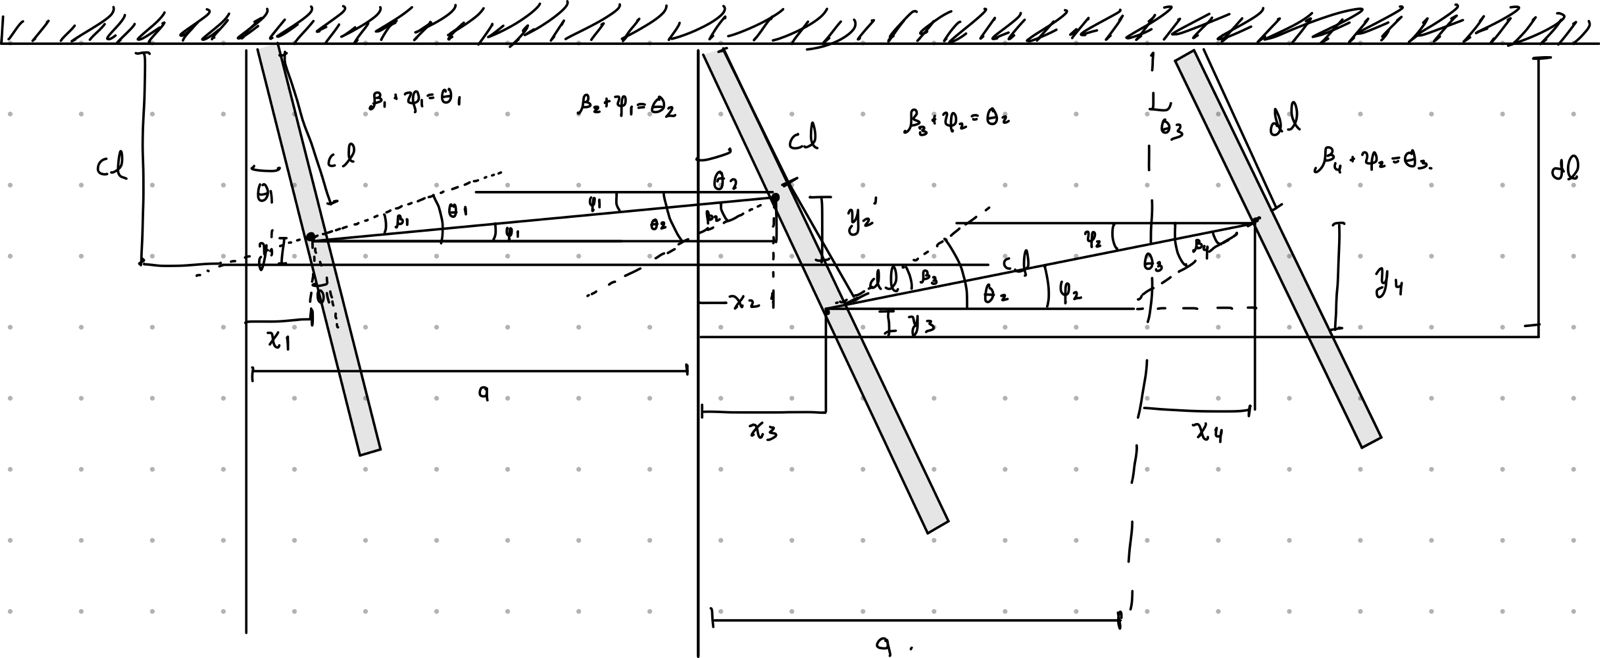
\includegraphics[width=0.75\textwidth, keepaspectratio]{Figures/IM1.jpeg}
    \caption{Sistema de tres péndulos físicos acoplados por resortes.}
    \label{fig:sistema_pendulos}
\end{figure}


Donde el resultado de la sumatoria de torques para cada péndulo genera el siguiente sistema de ecuaciones:

\begin{equation}
\begin{aligned}
  \ddot{\theta}_1 =\; & \theta_1 \left( \frac{(cl)^2 - x_{cm1} m_1 g}{I_1} \right) + \theta_2 \left( -\frac{k_1 (cl)^2}{I_1} \right) \\
  \ddot{\theta}_2 =\; & \theta_1 \left( \frac{k_1 (cl)^2}{I_2} \right) + \theta_2 \left( -\frac{k_1 (cl)^2}{I_2} + \frac{k_2 (dl)^2}{I_2} + \frac{x_{cm2} m_2 g}{I_2} \right) + \theta_3 \left( \frac{k_2 (dl)^2}{I_2} \right) \\
  \ddot{\theta}_3 =\; & \theta_2 \left( \frac{k_2 (dl)^2}{I_3} \right) + \theta_3 \left( -\frac{k_2 (dl)^2}{I_3} - \frac{x_{cm3} m_3 g}{I_3} \right)
\end{aligned}
\end{equation}